\documentclass[twoside]{book}

% Packages required by doxygen
\usepackage{fixltx2e}
\usepackage{calc}
\usepackage{doxygen}
\usepackage[export]{adjustbox} % also loads graphicx
\usepackage{graphicx}
\usepackage[utf8]{inputenc}
\usepackage{makeidx}
\usepackage{multicol}
\usepackage{multirow}
\PassOptionsToPackage{warn}{textcomp}
\usepackage{textcomp}
\usepackage[nointegrals]{wasysym}
\usepackage[table]{xcolor}

% NLS support packages
\usepackage[spanish]{babel}
% Font selection
\usepackage[T1]{fontenc}
\usepackage[scaled=.90]{helvet}
\usepackage{courier}
\usepackage{amssymb}
\usepackage{sectsty}
\renewcommand{\familydefault}{\sfdefault}
\allsectionsfont{%
  \fontseries{bc}\selectfont%
  \color{darkgray}%
}
\renewcommand{\DoxyLabelFont}{%
  \fontseries{bc}\selectfont%
  \color{darkgray}%
}
\newcommand{\+}{\discretionary{\mbox{\scriptsize$\hookleftarrow$}}{}{}}

% Page & text layout
\usepackage{geometry}
\geometry{%
  a4paper,%
  top=2.5cm,%
  bottom=2.5cm,%
  left=2.5cm,%
  right=2.5cm%
}
\tolerance=750
\hfuzz=15pt
\hbadness=750
\setlength{\emergencystretch}{15pt}
\setlength{\parindent}{0cm}
\setlength{\parskip}{3ex plus 2ex minus 2ex}
\makeatletter
\renewcommand{\paragraph}{%
  \@startsection{paragraph}{4}{0ex}{-1.0ex}{1.0ex}{%
    \normalfont\normalsize\bfseries\SS@parafont%
  }%
}
\renewcommand{\subparagraph}{%
  \@startsection{subparagraph}{5}{0ex}{-1.0ex}{1.0ex}{%
    \normalfont\normalsize\bfseries\SS@subparafont%
  }%
}
\makeatother

% Headers & footers
\usepackage{fancyhdr}
\pagestyle{fancyplain}
\fancyhead[LE]{\fancyplain{}{\bfseries\thepage}}
\fancyhead[CE]{\fancyplain{}{}}
\fancyhead[RE]{\fancyplain{}{\bfseries\leftmark}}
\fancyhead[LO]{\fancyplain{}{\bfseries\rightmark}}
\fancyhead[CO]{\fancyplain{}{}}
\fancyhead[RO]{\fancyplain{}{\bfseries\thepage}}
\fancyfoot[LE]{\fancyplain{}{}}
\fancyfoot[CE]{\fancyplain{}{}}
\fancyfoot[RE]{\fancyplain{}{\bfseries\scriptsize Generado por Doxygen }}
\fancyfoot[LO]{\fancyplain{}{\bfseries\scriptsize Generado por Doxygen }}
\fancyfoot[CO]{\fancyplain{}{}}
\fancyfoot[RO]{\fancyplain{}{}}
\renewcommand{\footrulewidth}{0.4pt}
\renewcommand{\chaptermark}[1]{%
  \markboth{#1}{}%
}
\renewcommand{\sectionmark}[1]{%
  \markright{\thesection\ #1}%
}

% Indices & bibliography
\usepackage{natbib}
\usepackage[titles]{tocloft}
\setcounter{tocdepth}{3}
\setcounter{secnumdepth}{5}
\makeindex

% Hyperlinks (required, but should be loaded last)
\usepackage{ifpdf}
\ifpdf
  \usepackage[pdftex,pagebackref=true]{hyperref}
\else
  \usepackage[ps2pdf,pagebackref=true]{hyperref}
\fi
\hypersetup{%
  colorlinks=true,%
  linkcolor=blue,%
  citecolor=blue,%
  unicode%
}

% Custom commands
\newcommand{\clearemptydoublepage}{%
  \newpage{\pagestyle{empty}\cleardoublepage}%
}

\usepackage{caption}
\captionsetup{labelsep=space,justification=centering,font={bf},singlelinecheck=off,skip=4pt,position=top}

%===== C O N T E N T S =====

\begin{document}

% Titlepage & ToC
\hypersetup{pageanchor=false,
             bookmarksnumbered=true,
             pdfencoding=unicode
            }
\pagenumbering{roman}
\begin{titlepage}
\vspace*{7cm}
\begin{center}%
{\Large L\+A\+N\+G\+U\+A\+G\+ES A\+ND W\+O\+RD L\+I\+S\+TS \\[1ex]\large 0 }\\
\vspace*{1cm}
{\large Generado por Doxygen 1.8.11}\\
\end{center}
\end{titlepage}
\clearemptydoublepage
\tableofcontents
\clearemptydoublepage
\pagenumbering{arabic}
\hypersetup{pageanchor=true}

%--- Begin generated contents ---
\chapter{Índice de clases}
\section{Lista de clases}
Lista de las clases, estructuras, uniones e interfaces con una breve descripción\+:\begin{DoxyCompactList}
\item\contentsline{section}{\hyperlink{classLanguage}{Language} \\*Class fully implemented. It is used to store and manage all the details concerning a given language. It includes and make it publicily available some functions in wordlist.\+h like those to change the encoding of characters. {\bfseries All the characters stored in memory use the I\+S\+O8859 standard} but characters read from keyboard might follow the U\+TF standard. These functions allow to change from one to another }{\pageref{classLanguage}}{}
\end{DoxyCompactList}

\chapter{Indice de archivos}
\section{Lista de archivos}
Lista de todos los archivos documentados y con descripciones breves\+:\begin{DoxyCompactList}
\item\contentsline{section}{include/\hyperlink{language_8h}{language.\+h} \\*Fully functional static library to handle languages, which are represented as a full list of allowed words, stored as a tree to make search efficient O(n) being n the number of letters in the word to be loocked up }{\pageref{language_8h}}{}
\item\contentsline{section}{src/\hyperlink{language_8cpp}{language.\+cpp} \\*Fully functional static library to handle languages, which are represented as a full list of allowed words, stored as a tree to make search efficient O(n) being n the number of letters in the word to be loocked up }{\pageref{language_8cpp}}{}
\end{DoxyCompactList}

\chapter{Documentación de las clases}
\hypertarget{classLanguage}{}\section{Referencia de la Clase Language}
\label{classLanguage}\index{Language@{Language}}


Class fully implemented. It is used to store and manage all the details concerning a given language. It includes and make it publicily available some functions in wordlist.\+h like those to change the encoding of characters. {\bfseries All the characters stored in memory use the I\+S\+O8859 standard} but characters read from keyboard might follow the U\+TF standard. These functions allow to change from one to another.  




{\ttfamily \#include $<$language.\+h$>$}

\subsection*{Métodos públicos}
\begin{DoxyCompactItemize}
\item 
\hyperlink{classLanguage_a09448361f9188bceaaeebc5576cd6896}{Language} ()\hypertarget{classLanguage_a09448361f9188bceaaeebc5576cd6896}{}\label{classLanguage_a09448361f9188bceaaeebc5576cd6896}

\begin{DoxyCompactList}\small\item\em Basic constructor and initializer. \end{DoxyCompactList}\item 
\hyperlink{classLanguage_ad7c92d28e44058ef4c7ea1b413a4b269}{Language} (std\+::string language)
\begin{DoxyCompactList}\small\item\em Basic constructor and initializer. \end{DoxyCompactList}\item 
bool \hyperlink{classLanguage_a677a05e98da32c5c54b6bf6343f80e21}{query} (std\+::string word) const 
\begin{DoxyCompactList}\small\item\em Query if a given word exists in the given language. \end{DoxyCompactList}\item 
std\+::string \hyperlink{classLanguage_ac78d5ca1b8305425b3343b53dca48b25}{get\+Language} () const 
\begin{DoxyCompactList}\small\item\em Returns the I\+S\+O690 identifier of the language. \end{DoxyCompactList}\item 
void \hyperlink{classLanguage_accc1c22d8bba3002a71bea06cecf624b}{set\+Language} (std\+::string lang)
\begin{DoxyCompactList}\small\item\em Loads the chosen language, which must be under $<$root$>$/languages folder. \end{DoxyCompactList}\item 
int \hyperlink{classLanguage_a39a391f8edca1cbdfeea606d968f2c4a}{get\+Frequency} (char letter) const 
\begin{DoxyCompactList}\small\item\em Query the frecuency of appearance in Scrabble of the given letter, according to the chosen language. \end{DoxyCompactList}\item 
int \hyperlink{classLanguage_aa750e6f524fc6a51d0ef82dee5826fbf}{get\+Score} (char letter) const 
\begin{DoxyCompactList}\small\item\em Query the score in Scrabble of the given letter, according to the chosen language. \end{DoxyCompactList}\item 
std\+::string \hyperlink{classLanguage_a8c26af3042d9808963f05450f2d28f7e}{get\+Letter\+Set} () const 
\begin{DoxyCompactList}\small\item\em Query the full set of available letters (without repetitions) in a given language. \end{DoxyCompactList}\end{DoxyCompactItemize}


\subsection{Descripción detallada}
Class fully implemented. It is used to store and manage all the details concerning a given language. It includes and make it publicily available some functions in wordlist.\+h like those to change the encoding of characters. {\bfseries All the characters stored in memory use the I\+S\+O8859 standard} but characters read from keyboard might follow the U\+TF standard. These functions allow to change from one to another. 


\begin{DoxyItemize}
\item std\+::string I\+S\+O8859to\+U\+T\+F8(const char $\ast$ in);
\item std\+::string U\+T\+F8to\+I\+S\+O8859(const char $\ast$ in);
\end{DoxyItemize}

{\bfseries Please note that all characters are stored in uppercase} 

Definición en la línea 27 del archivo language.\+h.



\subsection{Documentación del constructor y destructor}
\index{Language@{Language}!Language@{Language}}
\index{Language@{Language}!Language@{Language}}
\subsubsection[{\texorpdfstring{Language(std\+::string language)}{Language(std::string language)}}]{\setlength{\rightskip}{0pt plus 5cm}Language\+::\+Language (
\begin{DoxyParamCaption}
\item[{std\+::string}]{language}
\end{DoxyParamCaption}
)}\hypertarget{classLanguage_ad7c92d28e44058ef4c7ea1b413a4b269}{}\label{classLanguage_ad7c92d28e44058ef4c7ea1b413a4b269}


Basic constructor and initializer. 


\begin{DoxyParams}{Parámetros}
{\em language} & \hyperlink{classLanguage}{Language} chosen according to international rules I\+S\+O639-\/1 \href{https://en.wikipedia.org/wiki/List_of_ISO_639-1_codes}{\tt https\+://en.\+wikipedia.\+org/wiki/\+List\+\_\+of\+\_\+\+I\+S\+O\+\_\+639-\/1\+\_\+codes} \\
\hline
\end{DoxyParams}
\begin{DoxyNote}{Nota}
If the language chosen does not exists in the folder $<$root$>$/languages it throws an exception and stops the program 
\end{DoxyNote}


\subsection{Documentación de las funciones miembro}
\index{Language@{Language}!get\+Frequency@{get\+Frequency}}
\index{get\+Frequency@{get\+Frequency}!Language@{Language}}
\subsubsection[{\texorpdfstring{get\+Frequency(char letter) const }{getFrequency(char letter) const }}]{\setlength{\rightskip}{0pt plus 5cm}int Language\+::get\+Frequency (
\begin{DoxyParamCaption}
\item[{char}]{letter}
\end{DoxyParamCaption}
) const}\hypertarget{classLanguage_a39a391f8edca1cbdfeea606d968f2c4a}{}\label{classLanguage_a39a391f8edca1cbdfeea606d968f2c4a}


Query the frecuency of appearance in Scrabble of the given letter, according to the chosen language. 


\begin{DoxyParams}{Parámetros}
{\em letter} & The letter to query \\
\hline
\end{DoxyParams}
\begin{DoxyReturn}{Devuelve}
The frequency of appearance of the letter in the Scrabble of the given language. It returns 
\end{DoxyReturn}

\begin{DoxyRetVals}{Valores devueltos}
{\em 0} & if the letter does not appear in the language \\
\hline
\end{DoxyRetVals}


Definición en la línea 69 del archivo language.\+cpp.

\index{Language@{Language}!get\+Language@{get\+Language}}
\index{get\+Language@{get\+Language}!Language@{Language}}
\subsubsection[{\texorpdfstring{get\+Language() const }{getLanguage() const }}]{\setlength{\rightskip}{0pt plus 5cm}string Language\+::get\+Language (
\begin{DoxyParamCaption}
{}
\end{DoxyParamCaption}
) const}\hypertarget{classLanguage_ac78d5ca1b8305425b3343b53dca48b25}{}\label{classLanguage_ac78d5ca1b8305425b3343b53dca48b25}


Returns the I\+S\+O690 identifier of the language. 

\begin{DoxyReturn}{Devuelve}
A string with the ID of the language \href{https://en.wikipedia.org/wiki/List_of_ISO_639-1_codes}{\tt https\+://en.\+wikipedia.\+org/wiki/\+List\+\_\+of\+\_\+\+I\+S\+O\+\_\+639-\/1\+\_\+codes} 
\end{DoxyReturn}


Definición en la línea 65 del archivo language.\+cpp.

\index{Language@{Language}!get\+Letter\+Set@{get\+Letter\+Set}}
\index{get\+Letter\+Set@{get\+Letter\+Set}!Language@{Language}}
\subsubsection[{\texorpdfstring{get\+Letter\+Set() const }{getLetterSet() const }}]{\setlength{\rightskip}{0pt plus 5cm}string Language\+::get\+Letter\+Set (
\begin{DoxyParamCaption}
{}
\end{DoxyParamCaption}
) const}\hypertarget{classLanguage_a8c26af3042d9808963f05450f2d28f7e}{}\label{classLanguage_a8c26af3042d9808963f05450f2d28f7e}


Query the full set of available letters (without repetitions) in a given language. 

\begin{DoxyReturn}{Devuelve}
A string containing the letters available in I\+S\+O8859 
\end{DoxyReturn}


Definición en la línea 84 del archivo language.\+cpp.

\index{Language@{Language}!get\+Score@{get\+Score}}
\index{get\+Score@{get\+Score}!Language@{Language}}
\subsubsection[{\texorpdfstring{get\+Score(char letter) const }{getScore(char letter) const }}]{\setlength{\rightskip}{0pt plus 5cm}int Language\+::get\+Score (
\begin{DoxyParamCaption}
\item[{char}]{letter}
\end{DoxyParamCaption}
) const}\hypertarget{classLanguage_aa750e6f524fc6a51d0ef82dee5826fbf}{}\label{classLanguage_aa750e6f524fc6a51d0ef82dee5826fbf}


Query the score in Scrabble of the given letter, according to the chosen language. 


\begin{DoxyParams}{Parámetros}
{\em letter} & The letter to query \\
\hline
\end{DoxyParams}
\begin{DoxyReturn}{Devuelve}
The number of points of the letter in the Scrabble of the given language. It returns 
\end{DoxyReturn}

\begin{DoxyRetVals}{Valores devueltos}
{\em 0} & if the letter does not appear in the language \\
\hline
\end{DoxyRetVals}


Definición en la línea 76 del archivo language.\+cpp.

\index{Language@{Language}!query@{query}}
\index{query@{query}!Language@{Language}}
\subsubsection[{\texorpdfstring{query(std\+::string word) const }{query(std::string word) const }}]{\setlength{\rightskip}{0pt plus 5cm}bool Language\+::query (
\begin{DoxyParamCaption}
\item[{std\+::string}]{word}
\end{DoxyParamCaption}
) const}\hypertarget{classLanguage_a677a05e98da32c5c54b6bf6343f80e21}{}\label{classLanguage_a677a05e98da32c5c54b6bf6343f80e21}


Query if a given word exists in the given language. 


\begin{DoxyParams}{Parámetros}
{\em word} & The word to be queried \\
\hline
\end{DoxyParams}
\begin{DoxyReturn}{Devuelve}

\end{DoxyReturn}

\begin{DoxyRetVals}{Valores devueltos}
{\em true} & if the word exists in the recorded language, \\
\hline
{\em false} & otherwise \\
\hline
\end{DoxyRetVals}


Definición en la línea 61 del archivo language.\+cpp.

\index{Language@{Language}!set\+Language@{set\+Language}}
\index{set\+Language@{set\+Language}!Language@{Language}}
\subsubsection[{\texorpdfstring{set\+Language(std\+::string lang)}{setLanguage(std::string lang)}}]{\setlength{\rightskip}{0pt plus 5cm}void Language\+::set\+Language (
\begin{DoxyParamCaption}
\item[{std\+::string}]{lang}
\end{DoxyParamCaption}
)}\hypertarget{classLanguage_accc1c22d8bba3002a71bea06cecf624b}{}\label{classLanguage_accc1c22d8bba3002a71bea06cecf624b}


Loads the chosen language, which must be under $<$root$>$/languages folder. 


\begin{DoxyParams}{Parámetros}
{\em lang} & The ID of the language \\
\hline
\end{DoxyParams}
\begin{DoxyNote}{Nota}
If the language chosen does not exists in the folder $<$root$>$/languages it throws an exception and stops the program 
\end{DoxyNote}


Definición en la línea 26 del archivo language.\+cpp.



La documentación para esta clase fue generada a partir de los siguientes ficheros\+:\begin{DoxyCompactItemize}
\item 
include/\hyperlink{language_8h}{language.\+h}\item 
src/\hyperlink{language_8cpp}{language.\+cpp}\end{DoxyCompactItemize}

\chapter{Documentación de archivos}
\hypertarget{language_8h}{}\section{Referencia del Archivo include/language.h}
\label{language_8h}\index{include/language.\+h@{include/language.\+h}}


Fully functional static library to handle languages, which are represented as a full list of allowed words, stored as a tree to make search efficient O(n) being n the number of letters in the word to be loocked up.  


{\ttfamily \#include $<$vector$>$}\\*
{\ttfamily \#include \char`\"{}wordlist.\+h\char`\"{}}\\*
Dependencia gráfica adjunta para language.\+h\+:\nopagebreak
\begin{figure}[H]
\begin{center}
\leavevmode
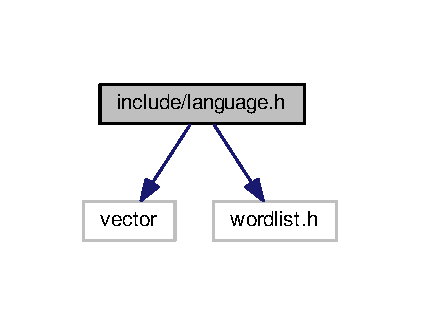
\includegraphics[width=202pt]{language_8h__incl}
\end{center}
\end{figure}
Gráfico de los archivos que directa o indirectamente incluyen a este archivo\+:\nopagebreak
\begin{figure}[H]
\begin{center}
\leavevmode
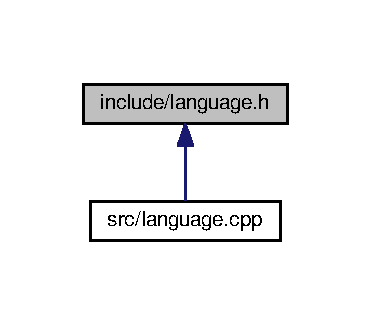
\includegraphics[width=178pt]{language_8h__dep__incl}
\end{center}
\end{figure}
\subsection*{Clases}
\begin{DoxyCompactItemize}
\item 
class \hyperlink{classLanguage}{Language}
\begin{DoxyCompactList}\small\item\em Class fully implemented. It is used to store and manage all the details concerning a given language. It includes and make it publicily available some functions in wordlist.\+h like those to change the encoding of characters. {\bfseries All the characters stored in memory use the I\+S\+O8859 standard} but characters read from keyboard might follow the U\+TF standard. These functions allow to change from one to another. \end{DoxyCompactList}\end{DoxyCompactItemize}


\subsection{Descripción detallada}
Fully functional static library to handle languages, which are represented as a full list of allowed words, stored as a tree to make search efficient O(n) being n the number of letters in the word to be loocked up. 

\begin{DoxyAuthor}{Autor}
D\+E\+C\+S\+AI 
\end{DoxyAuthor}
\begin{DoxyNote}{Nota}
Fully implemented. No further implementation required. 
\end{DoxyNote}

\hypertarget{language_8cpp}{}\section{Referencia del Archivo src/language.cpp}
\label{language_8cpp}\index{src/language.\+cpp@{src/language.\+cpp}}


Fully functional static library to handle languages, which are represented as a full list of allowed words, stored as a tree to make search efficient O(n) being n the number of letters in the word to be loocked up.  


{\ttfamily \#include $<$string$>$}\\*
{\ttfamily \#include $<$cassert$>$}\\*
{\ttfamily \#include $<$fstream$>$}\\*
{\ttfamily \#include $<$iostream$>$}\\*
{\ttfamily \#include \char`\"{}language.\+h\char`\"{}}\\*
Dependencia gráfica adjunta para language.\+cpp\+:\nopagebreak
\begin{figure}[H]
\begin{center}
\leavevmode
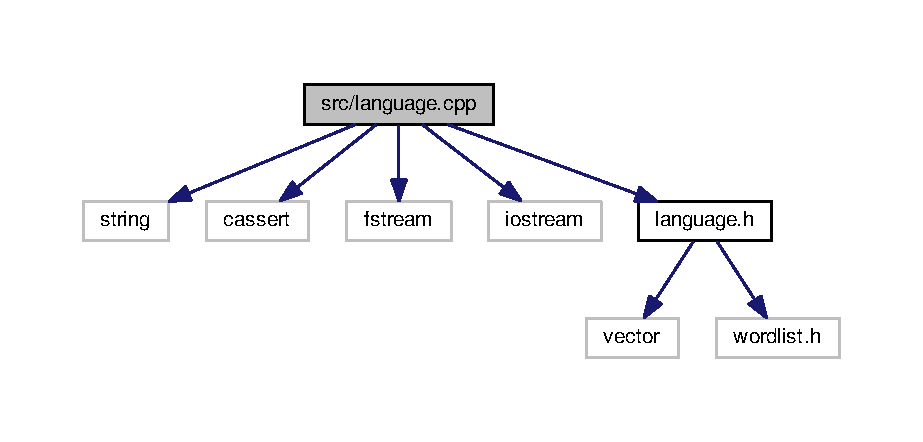
\includegraphics[width=350pt]{language_8cpp__incl}
\end{center}
\end{figure}


\subsection{Descripción detallada}
Fully functional static library to handle languages, which are represented as a full list of allowed words, stored as a tree to make search efficient O(n) being n the number of letters in the word to be loocked up. 

\begin{DoxyAuthor}{Autor}
D\+E\+C\+S\+AI 
\end{DoxyAuthor}
\begin{DoxyNote}{Nota}
Fully implemented. No further implementation required. 
\end{DoxyNote}

%--- End generated contents ---

% Index
\backmatter
\newpage
\phantomsection
\clearemptydoublepage
\addcontentsline{toc}{chapter}{Índice}
\printindex

\end{document}
